\chapter{Particle Reconstruction at CMS}
\label{reconstruction_overview}

\par Charged and neutral hadrons in the form of jets, missing
transverse energy (MET), photons, electrons, muons, and tau leptons
are reconstructed at CMS using the particle flow event-reconstruction
algorithm \cite{CMS-PAS-PFT-09-001}.  The algorithm is based on on a
three step process of identifying charged particle tracks using the
muon chambers and silicontracker, identifying clusters of energy in
the ECAL and HCAL, and linking the tracks to the calorimeter
clusters.  The calorimeter energy deposits were calibrated with test
beam sources, data from cosmic rays and beam dumps, and finally from
collision data.  The algorithm constructs muons by fitting the tracks
formed between the muon chambers, pixel and silicon trackers.
Electrons have tracks from the pixel and silicon tracker matched to
the ECAL, with a minimum energy deposited in the HCAL.  Jets are
formed from tracks, ECAL, and HCAL clusters falling with a conical
angle.  The identification of one, three, or larger odd number of
tracks, and the majoriy of the energy contained in a small cone size,
allows a jet to be tagged as a hadronically decaying tau lepton.
Additional algorithms are also used to identrify a jet as coming from
the decay of a b-quark, primarily by looking for secondary vertices in
the pixel and silicon tracker.  


\section{Iterative Tracking}
\label{iterative_tracking_overview}

\par Since approximately two-thirds of the energy of a jet is carried by
charged hadrons, the tracker is the cornerstone of the particle-flow
algorthm \cite{CMS-PAS-PFT-09-001}.  The path of a charged particle in
a magnetic field follows a helical pattern, described by 5 parameters.
The extraction of these requires three 3-dimensional measurements of
the particle, or two 3-dimensional measurements and a constraint on
the origin \cite{Chatrchyan:2014fea}.  The pixel detector is ideal for
this since each pixel provides a 3-dimensional measurment of the
particle's location.  Track reconstruction is the process of using
hits in the pixel and silicon detector elements to estimate the
momentum and trajectory of the charged particle  responsible for the
hit \cite{Chatrchyan:2014fea}.  The tracking software at CMS is known
as the Combinatorial Track Finder (CTF), which is based on producing
tracks over multiple iterations of the reconstruction sequence,
removing the tracks with the largest \PT closest to the interaction
region first, reducing the combinatorial complexity over each
iteration.   

\par Each iteration begins by identifying a seed for the particle
tracks, which is a minimum combination of pixel or silicon tracker
hits that is used as an initial estimate of the trajectory of the
particle \cite{Chatrchyan:2014fea}.  Then, tracks are found by applying
the Kalman filter \cite{Fruhwirth:1987fm}.  This method is based on
applying a small guassian uncertainty to the location of the seed
hits, fitting an intial track to these hits, then looking for
additional hits that fall within the error of the initial estimate,
deeper in the tracker.  These hits are added to the fit with their own
uncertainties, and the fit is re-calculated, each time attempting to
minimize the mean-square estimation of the error.  The 5 helical
trajectory parameters are extracted, and tracks with poor fits are
discarded.    

\par A total a six iterations is used, each with a different starting
seed or kinematic requirement on the \PT of the tack, as well as
the transverse and longitudinal distance from the reconstructed
vertex \cite{Fruhwirth:1987fm}.  The first iteration is seeded by
three hits in the pixel detector.  The second, is seeded by two hits
in the pixel detector and a pixel vertex, which is form when at least
four pixel tracks point back to a common origin.  The third iteration
is seeded once again by three hits in the pixel detector, except with
a looser minimum \PT cut.  The fourth iteration uses seeds from any
three hits in the pixel detector or silicon tracker, with at least one
hit coming from the pixel detector.  In the fifith iteration seeds are
formed from the inner two rings of the TIB, TID, and TEC.  The final
iteration begins with seeds from the first two rings of the TOB and
the fifth ring of the TEC.   


\section{Calorimeter Clustering}
\label{calorimeter_clustering_overview}

\par The clustering algorithm is used to detector the energy and
director of stable, neutral particles such as photons and neutral
hadrons \cite{CMS-PAS-PFT-09-001}.  It also seperates the energy
contributions from the netural and charged hadrons, and provides an
aditional energy measurement for charged hadrons with very low or high
\PT tracks, both cases that degrade the energy resolution.  Finally,
the clustering algorith properly accounts for bremmstrahlung energy
losses from electrons. The algorithm is performed independently for
the ECAL barrel, ECAL endcaps, HCAL barrel, and HCAL endcaps.  In the
HF, no clustering algorithms are used, as each cell is used as its own
cluster in an event.   

\par The clustering alorithm begins by identifying "cluster seeds'',
which are the highest \PT cells above a defined energy threshold
\cite{CMS-PAS-PFT-09-001}.  Then, "topological clusters'' are formed
by grouping adjacent cells together with energy above 80 MeV in the
ECAL barrel, 300 MeV in the ECAL endcaps, and 800 MeV in the HCAL.
As a new cell is added, the total cluster energy and position is
updated until no new cells are able to be added.  Each cluster seed
thus gives rise to a "particle-flow cluster''.  Each of these clusters
is used as a candidate to be associated with tracks during the third
stage of the algorithm, the linking step.  


\section{Calorimeter Energy Calibration}
\label{energy_calibration_overview}

\par One of the most critical steps in reconstructing particles is the
calorimeter energy calibration, which is the conversion of calormiter
scintillator light and photodetector current to the energy deposited
in the calorimeter by the particle traversing it.  This is done by
exposing the crystals to particles of a known energy, using large
samples of cosmic ray muons, by measuring minimum-bias events assuming
a $\phi$ symmetry, the of $\pi^{0}$ and$\eta^{0}$ meson resonances
decaying into photons, and $W$ and $Z$ bosons into electrons.   

\par Before installation at P5, the ECAL and HCAL were pre-calibrated
using test beam.  In 2006, the ECAL was exposed to an electron beam with
energies between 15 and 250 GeV \cite{Adzic:2008zza} at CERN.
Additionally, intercalibrations between crystals were perfored with 90
and 120 GeV beams.  Also at CERN in 2006, the HCAL was calibrated,
prior to installtion using a beam of 50 GeV pions
\cite{Cankocak:1127315}. 

\par Once both calorimeters were installed, the detectors were
calibrated with cosmic ray muon events in 2007 with the CMS magnet
de-energied during the CRUZET (Cosmic RUn at ZEro Tesla) data taking
campaign, and again with the CMS field on in 2008 during the CRAFT
(Cosmic Run At Four Tesla) campaign.  Shortly after the CRAFT
campaign, the LHC delivered 450 GeV proton beams to collimator targets
upstream of the CMS detector, creating accelerator muons that are
addtionally used to calibrate the detector respnse.  The ECAL encap
energy resolution was improved from 7.6$\%$ to 6.3$\%$, and in the
barrel, the intercalibrations from the test beam were validated at a
$2\%$ level of agreement \cite{Malberti:1358839}.  The HCAL energy
calibration resulted in 5$\%$ energy resolution in the HB, 10$\%$ in
the HE, $12\%$ in the HF, and $5\%$ in the
HE\cite{Chatrchyan:1223950}.  

\begin{figure}[h]
   \centering
  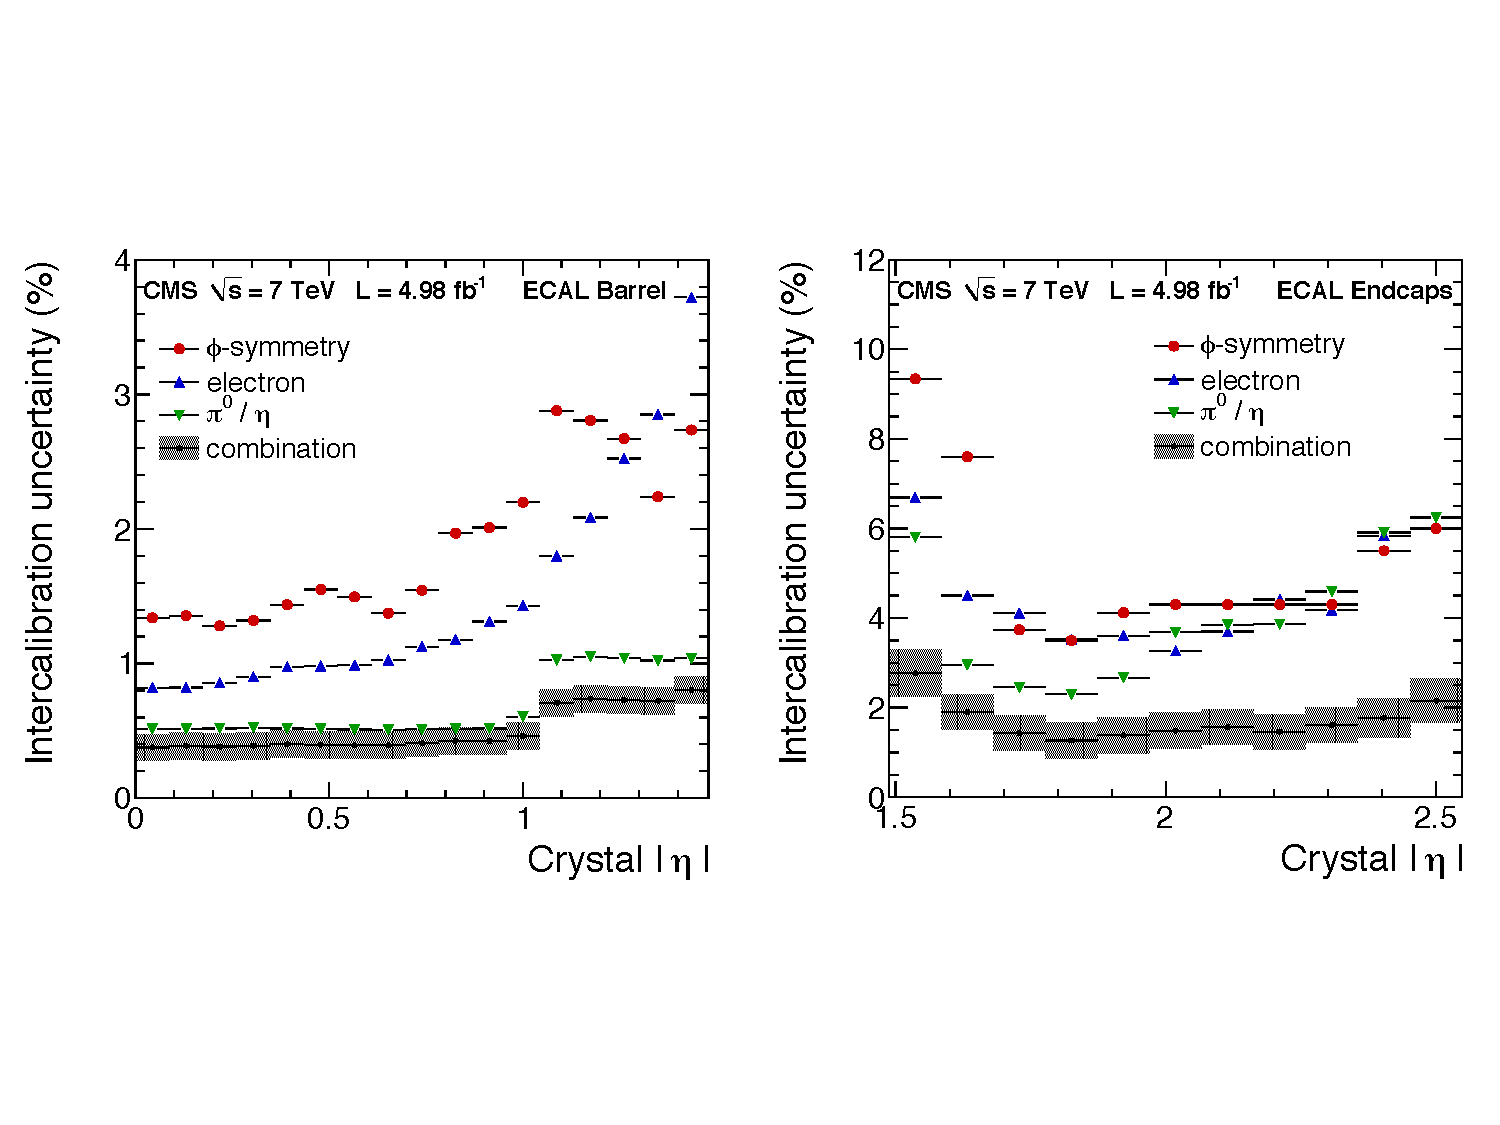
\includegraphics[width=0.9\textwidth]{Figures/Reconstruction_Diagrams/ECAL_intercalibration_combined_methods.pdf}
  \caption{Results of the uncertainty on the ECAL intercalibration
    coefficients for the barrel (left) and endcaps (right)} \label{fig:ecal_intercal}
\end{figure}

\par After an initial set of data collection three independent
calibration methods are combined to determine the absolute energy
scale and intercalibration coefficints for the crystals
\cite{Chatrchyan:155414}.  The first method uses a large amount of
data collected from minimum-bias trigger events, events which are
dominated by glancing collisions and QCD jet production.  The
processes that contribute to these events have final state particles
symmetrically distributed in the $\phi$ coordinate.  By grouping the
crystals into rings of $\eta$, and the response of each crystal can be
determined and modified such that it matches the average crystal
response in that $\eta$ ring, with the uncertainty on the average
representing the uncertainty on the intercalibraiton coefficient.  The
second method involves reconstructing the resonances of the $\pi^{0}$
and $\eta^{0}$ mesons decaying to two photons and relying on the
high-precision measurements from other experiment to determine the
exact mass of the resonance.  Events near the resonance of these two
particles are once again divided into rings of $\eta$, and averaged
over the $\phi$ coordinate.  Decays of the $Z$ boson an electron pair
is also used to determine the absolute scale (ADC counts/GeV) of the
crystals, once again relying on the higher-precsion measurements of
previous experiments for the location of the mass peak.  Finally,
comprisons between the energy measured in the tracker and that
measured in the ECAL are made from $W$ and $Z$ boson decays to a
electrons.  Figure \ref{fig:ecal_intercal} shows the results of
combining all three methods, to determine the uncertainty of the
intercalibration coefficients.  

\begin{figure}[h]
   \centering
  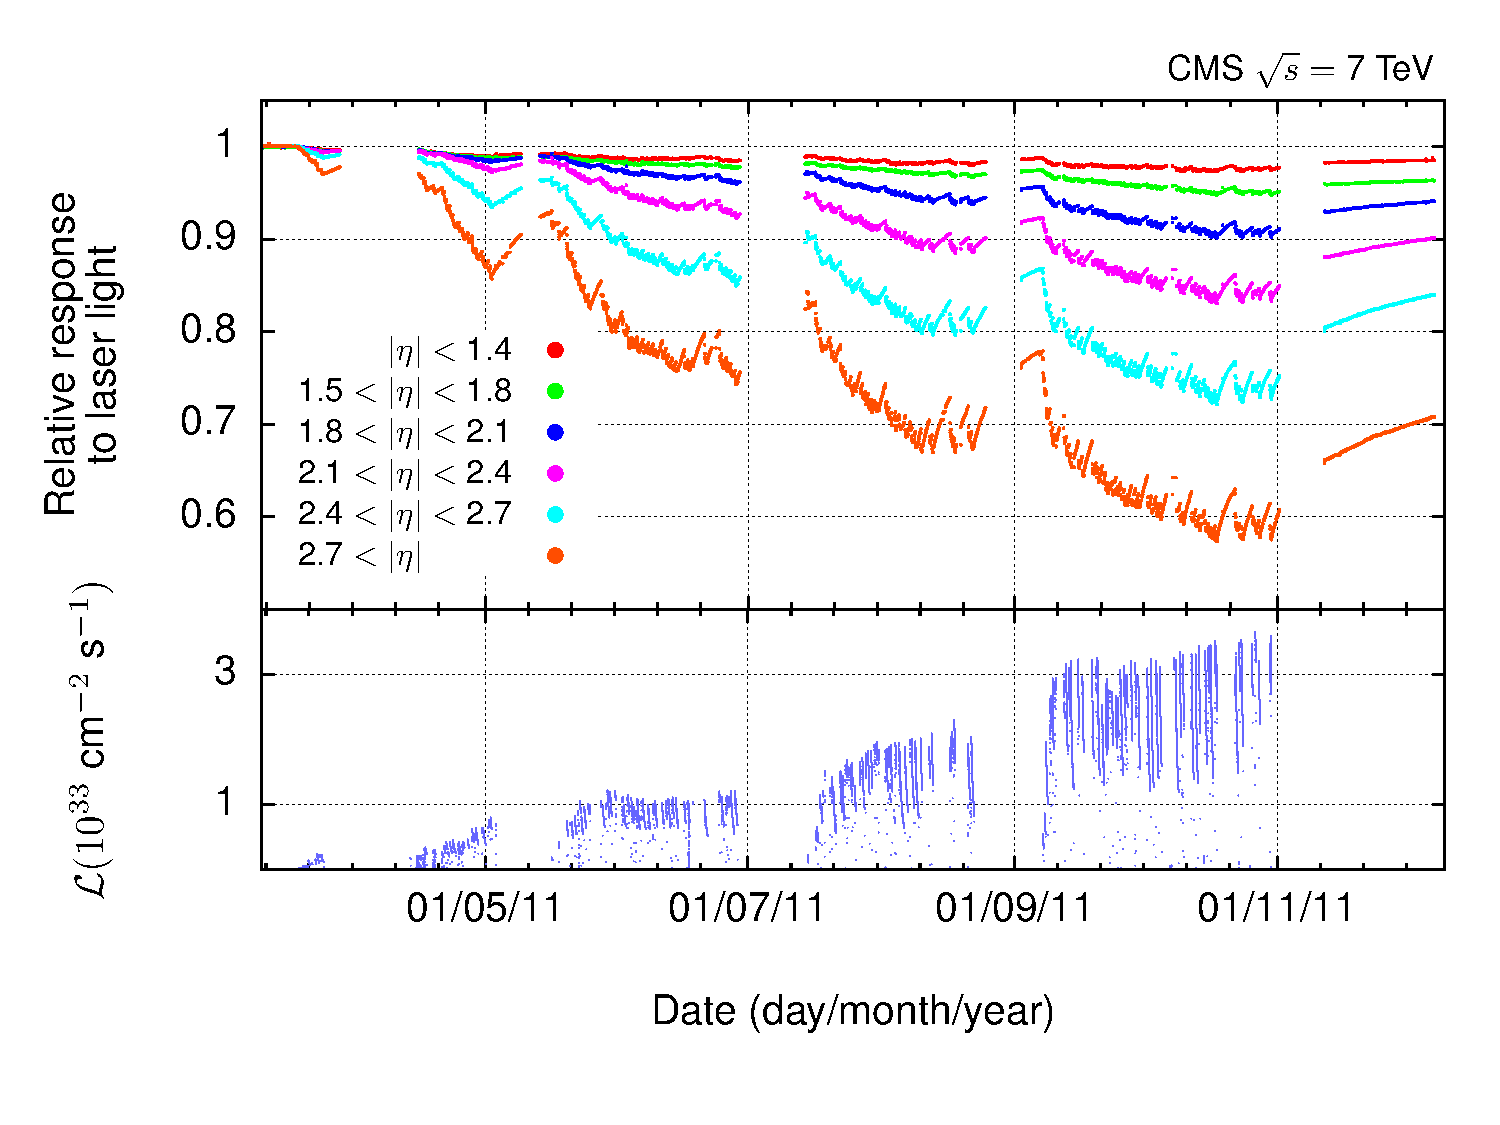
\includegraphics[width=0.9\textwidth]{Figures/Reconstruction_Diagrams/ECAL_inst_lumi_laser_calibration.pdf}
  \caption{Instaneous luminosity response to the crystals as measured
    by the laser and LED system.  Additional crystal calibration
    constants are derived to normalize the crystal reponse over the
    range of collected data} \label{fig:ecal_laser}
\end{figure}

\par The ECAL also has a strong dependence on the rate of
instantaneous luminosity that the crystals are exposed to.  It is
therefore necesary to perform additional crytal calibrations as a
function of time during a run of data collection.  Blue and orange
LED light, and blue laser light is fed through a network of optical
fibers to each crystal.  A known amount of light is injected and the
crystal response is measured.  Figure \ref{fig:ecal_laser} shows a
plot of the crystal response versus time.  Rings of $\eta$ are formed
and crystals within the same $\eta$ ring are used to calculated an
average response, as is done in the intercalibraiton procedures
described above.   

\begin{figure}[h]
   \centering
  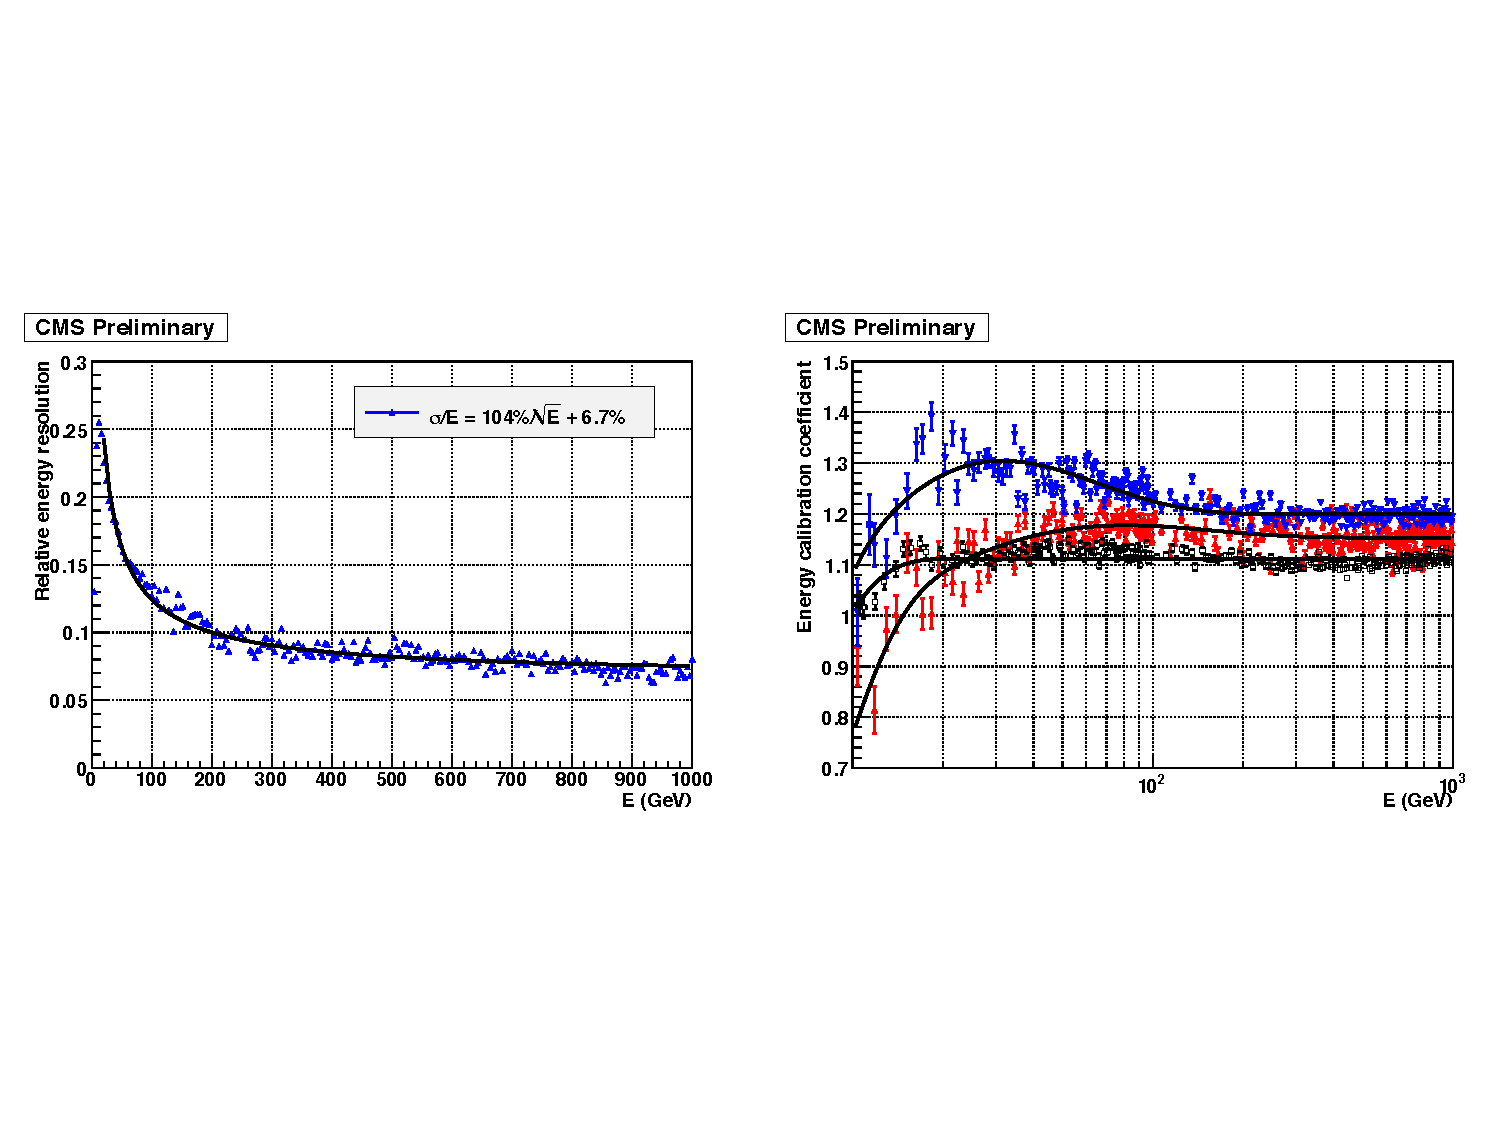
\includegraphics[width=0.9\textwidth]{Figures/Reconstruction_Diagrams/HCAL_calibration_chi2_fit_from_ecal.pdf}
  \caption{Results of using a $\chi^{2}$ minimization procedure to
    estimate the neutral hadron energy contribution in the HCAL using
    simulated events} \label{fig:hcal_calibration}
\end{figure}

\par The perfomance of the HCAL calibration to the 50 GeV pion beam is
validated by comparing energy measurements in the tracker to energy
deposits in the HCAL \cite{CMS-DP-2010-025}.  Since neutral hadrons
contribue approximately 10$\%$ of the energy contained in a jet, it is
necessary to recalibrate the measured energy in the HCAL using
simulated events where the true hadronic energy is known.  The
equation for the total calorimeter energy is given by:

\begin{equation}\label{eq:calorimeter_calibration}
E_{\text{calib}} = a + b(E, \eta)E_{ECAL} + c(E, \eta)E_{HCAL}
\end{equation} 

\noindent The coefficients, a, b, and c are determined through a
$\chi^{2}$ minimization procedure over each bin of energy, minimizing
the difference between the reconstructed and true energies and solving
for the parameters a, b, and c.  Figure \ref{fig:hcal_calibration}
shows the resulting HCAL energy resolution as a function of energy,
and the values of the coefficients a, b, and c.  


\section{Linking}
\label{linking_overview}

\par Once clusters are formed in the ECAL and HCAL barrels and
endcaps, they are associated with nearby tracks in the pixel and
silicon tracker in the phase of the particle-flow algorithm known as
linking \cite{CMS-PAS-PFT-09-001}.  Single particles are formed out of
the tracks and calorimeter clusters without double counting
contributions from different detectors, froming "blocks'' of linked
elements.  Due to the high granularity of each sub-detector, blocks of
two-four elements are typical.  

\par The linking procedure between pixel and silicon strip tracks and
the calorimeter deposits occurs in a three steps: extrapolting the
track to the ECAL preshower (PS); then to the ECAL to a depth
corresponding to the maximum longitudinal shower profile; and finally
to the HCAL to a depth corresponding to one interaction length.  A
track is then linked to a cluster if it falls within the cluster
boundaries.  One HCAL cluster may be associated to many tracks, but
each track can only be associated with a single cluster, determined as
the track with the shortest distance.  For the ECAL, one track may be
associated with many energy clusters, since they may have originated
from hadronic shower fluctuations, so links to tracks should be
preserved to avoid double counting the hadron energy.  In order to
account for the bremmstrahlung energy losses of electrons, tangent
lines to the tracks are linked to the ECAL.  If this extrapolated,
tangent track falls within the ECAL cluster boundaries, it becomes a
candidate for a bremmstrahlung photon from an electron.  Since the
ECAL has a finer granularity than the HCAL, clusters of the ECAL are
linked to HCAL clusters if an ECAL cluster falls within the boundary
of the HCAL cluster.   Finally, linking between the muon chambers and
the inner tracker occurs via a $\chi^{2}$ fit to a muon trajectory
that would traverse the entire detector.    

\section{Physics Object Reconstruction}
\label{physics_object_recostruction}

\par Once tracks have been formed from the muon chambers, pixel, and
silicon tracker detectors and linked to clusters in the ECAL and HCAL,
particles can be reconstructed.  The process begins by reconstructing
muons, then electrons and photons, finishing with charged and nuetral
hadrons.  The charged and neutral hadrons are then clusted together to
make jets, which can be tagged as $\tau$ or $b$-jets.  After each
object is formed, the tracks and calorimeter energy dpositions
associated with it are removed from the collection of blocks that are
used to form the particle-flow candidates, ensuring that no double
counting of energy contributions is taking place.  

\subsection{Muon Reconstruction}
\label{muon_reco_overview}

\par The reconstruction of physics objects in the particle-flow
algorithm begins by identifying muons \cite{CMS-PAS-PFT-09-001}.  The
algorithm begins by identying tracks in the pixel and silicon strip
detectors that have been linked to tracks in the muon chambers, and
fit with a muon trajectory with a minimum $\chi^{2}$.  Additionaly, it
is required that muon track that is fit with both muon chambers,
pixel, and silicon trakcer information is compatible within 3 sigma,
to a track fit with the pixel and silicon tracker information alone.
When the "particle-flow'' muon is removed from the collection of
candidate blocks, the muon tracks, and based on studies from the CRAFT
data run, 3 (0.5) GeV $\pm 100\%$ is removed from the HCAL (ECAL)
cells that the muon traverses.  

\begin{figure}{h}
    \centering
    \begin{subfigure}[h]{0.40\textwidth}
        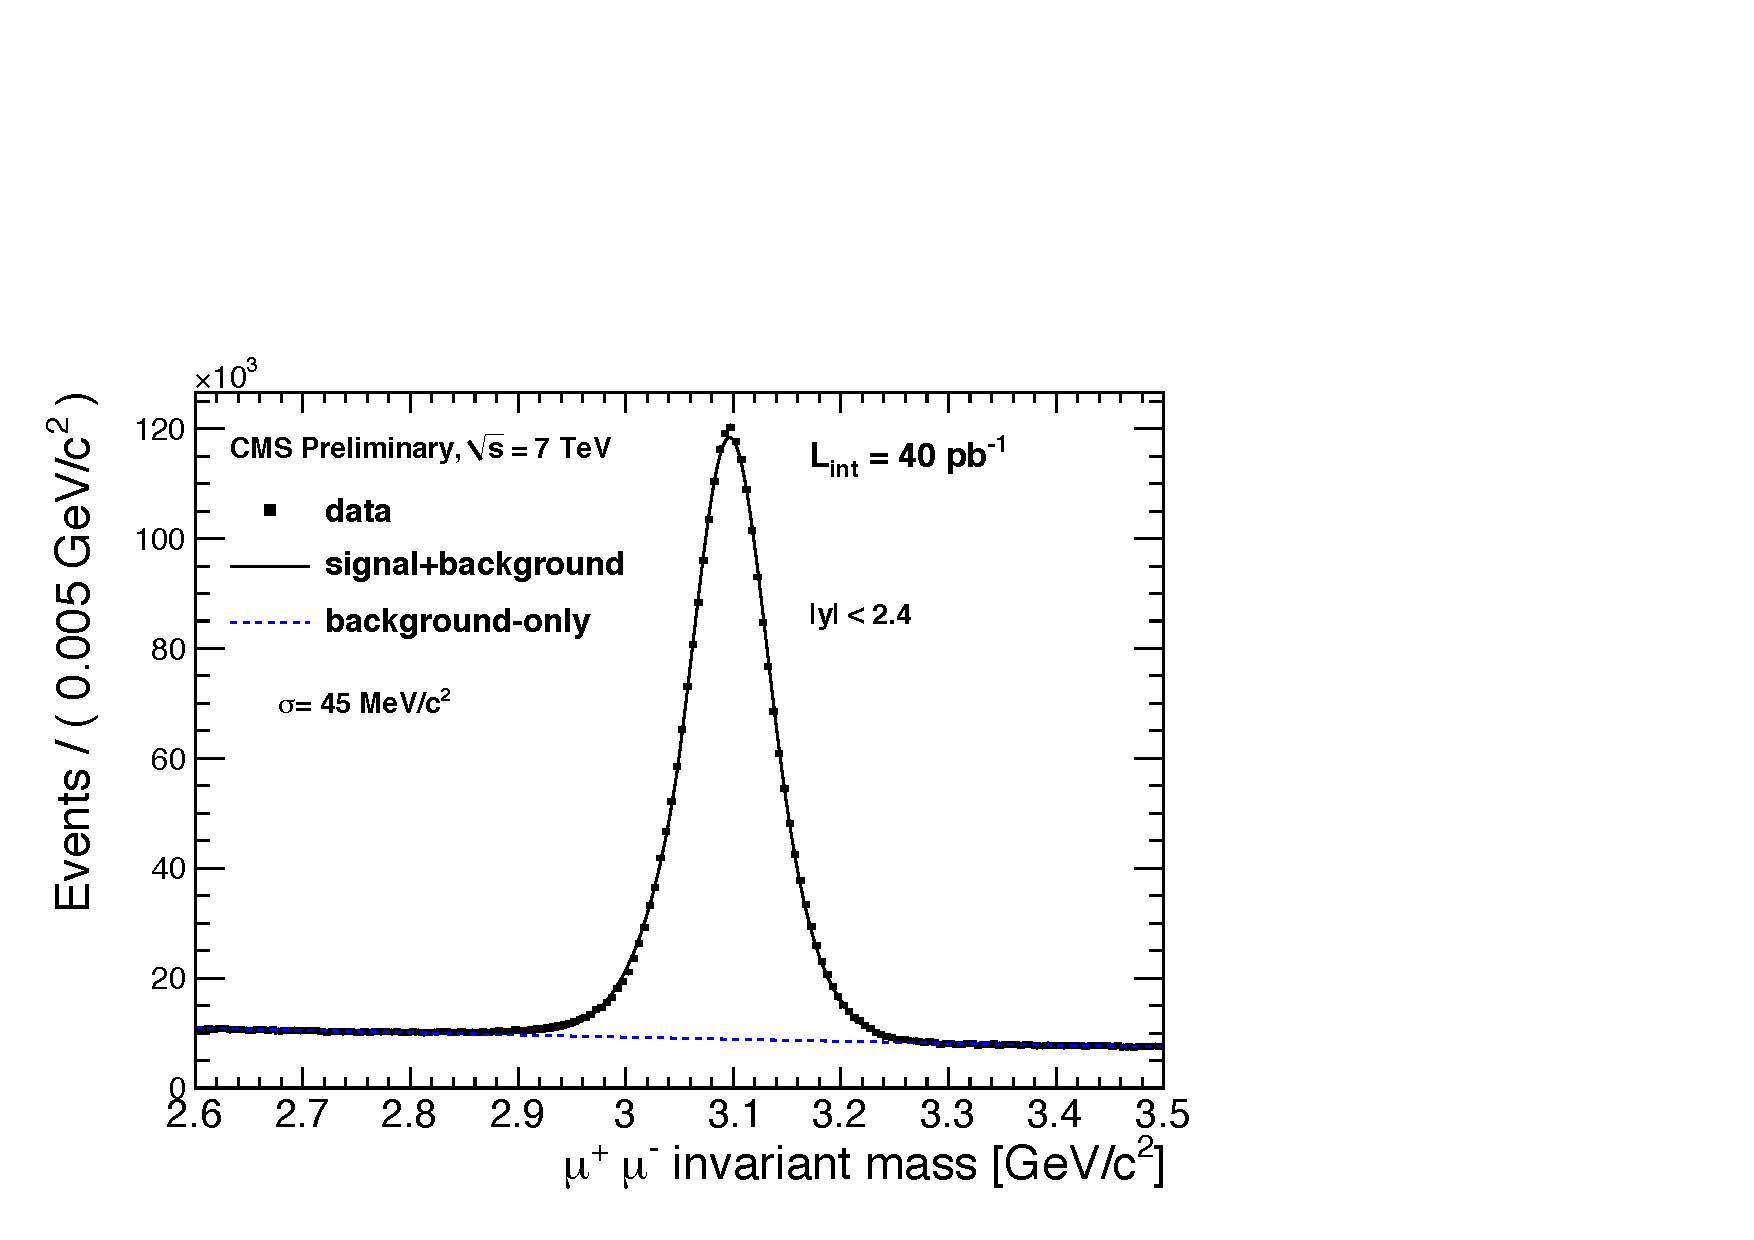
\includegraphics[width=\textwidth]{Figures/Reconstruction_Diagrams/MUO__JPsi40pb-1.pdf}
        \caption{Reconstructed J$\Psi$ mass peak from di-muon events
          in 7 TeV data, used to commision low \PT muons reconstructed
        with the particle flow algorithm}\label{fig:muon_jpsi_mass}
      \end{subfigure}
      ~ %add desired spacing between images, e. g. ~, \quad, \qquad, \hfill etc.
      % (or a blank line to force the subfigure onto a new line)
    \begin{subfigure}[h]{0.40\textwidth}
        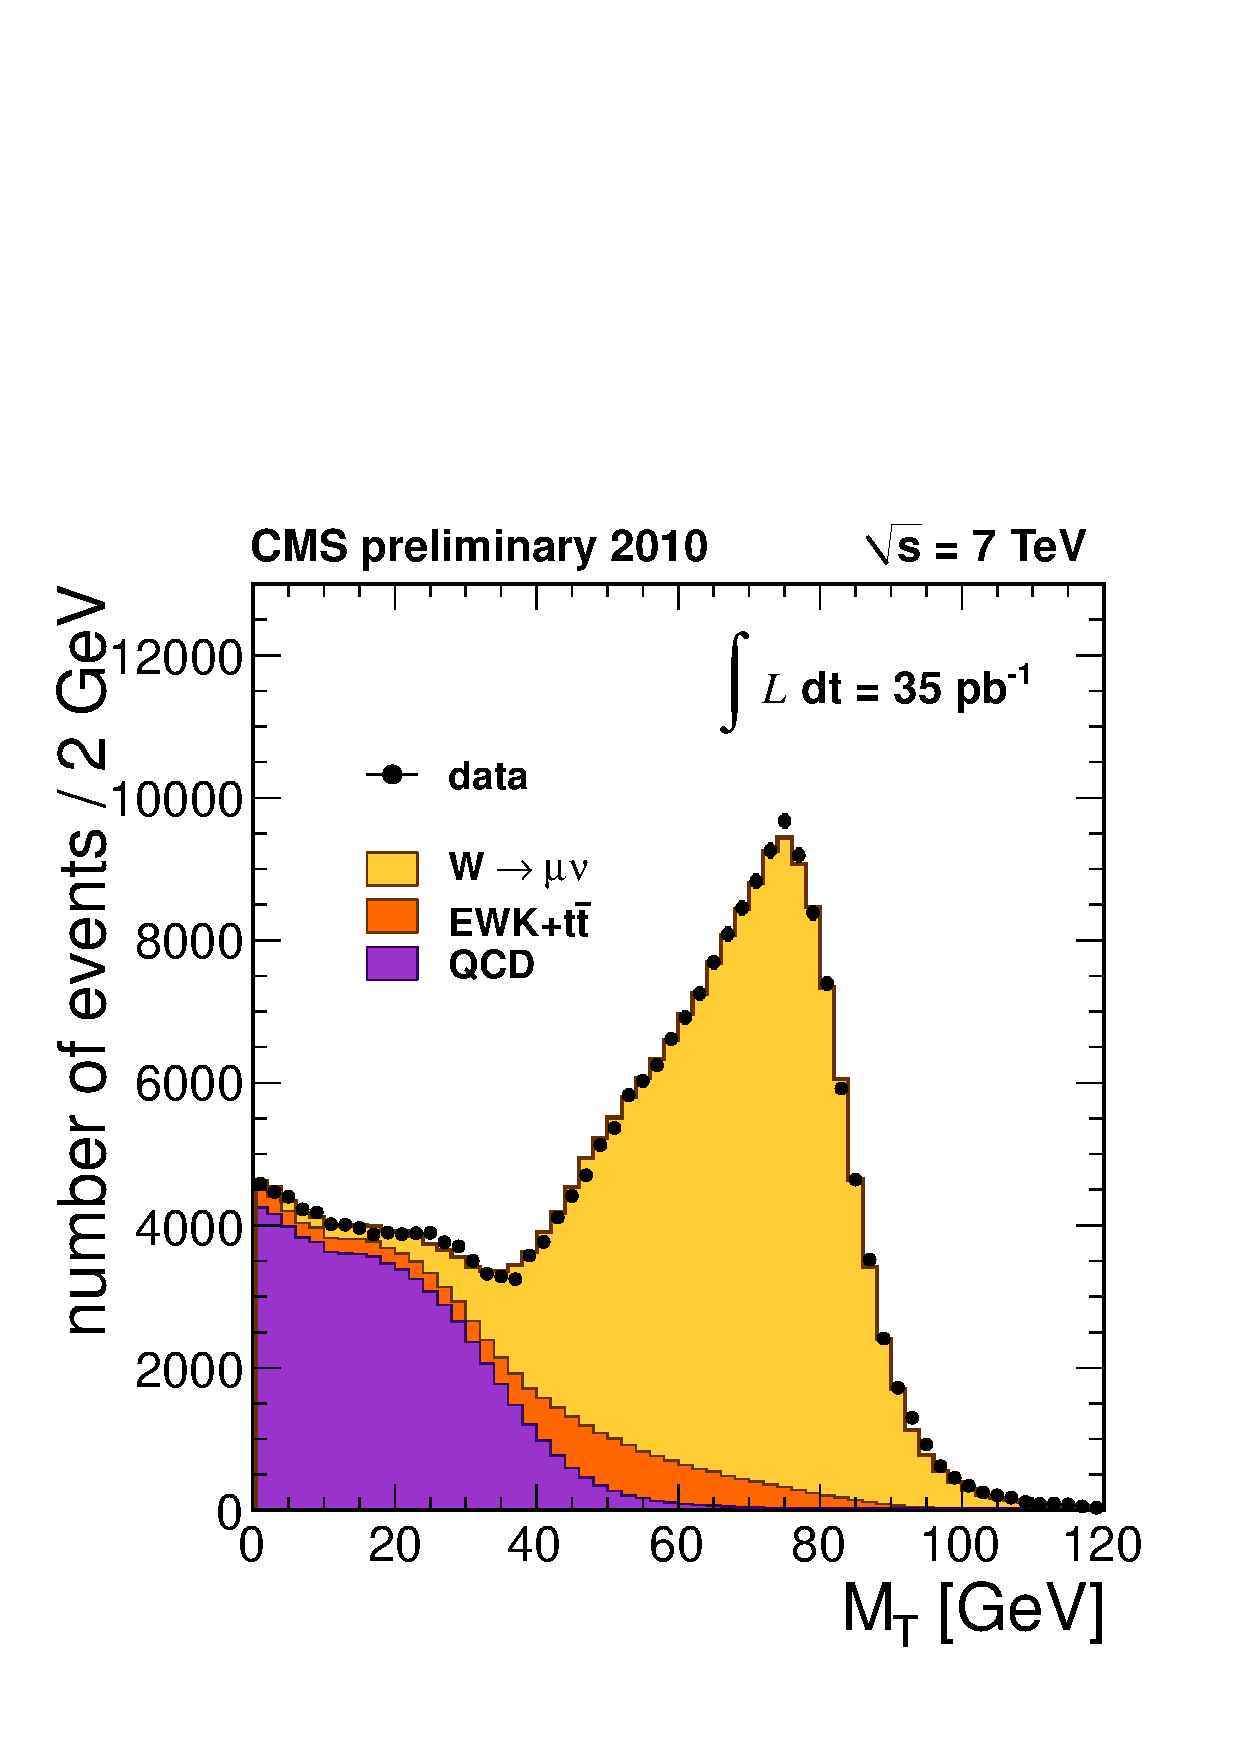
\includegraphics[width=\textwidth]{Figures/Reconstruction_Diagrams/MUO__Wmunu_35pb-1_lin.pdf}
        \caption{Transverse mass peak of $W$ boson events
          reconstructed from single muon events in 7 TeV data, used to
        commission high \PT muons reconstructed iwth the particle flow
      algorithm}\label{fig:muon_w_mass}
      \end{subfigure}
      \caption{Muon validation plots for the particle-flow reconstruction}\label{fig:muon_pf_validation}
\end{figure}

\par In 2010, 7 TeV data was collected \cite{CMS-PAS-PFT-10-003} in
order to commision the reconstruction of muons.  The J/$\Psi$
resonance at 3.1 GeV provides a large number of low \PT di-muon pairs.
Figure \ref{fig:muon_pf_validation}(\subref{fig:muon_jpsi_mass}) shows
the reconstructed J/$\Psi$ mass with 40 \pbinv of data.  High \PT
muons are commissioned by reconstructing the $W$ boson mass.  Figure
\ref{fig:muon_pf_validation}(\subref{fig:muon_w_mass}) shows the
results the first 35 \pbinv of 7 TeV data.   


\subsection{Electron Reconstruction}
\label{electron_reco_overview}

\par The next stage in particle-reconstruction is the identification
of electrons \cite{CMS-PAS-PFT-09-001}.  Electrons leaves hits in the
tracker and deposits most of its energy into the ECAL, with the
clustering widest in the $\phi$ direction due to brehmmstralung.
Electron tracks tend to be shorter and lose energy in the tracker do
to bremsmstrahlung, a highly non-linear process, that the Kalman
fitter used in the track identification phase is not optimized for.
These tracks are re-fit using the Guassian Sum Filter (GSF) algorithm
\cite{Adam:2005bya}. This algorithm accounts for the change in
trajectory of the electron due to bremmstrahlung, extending the
linking to ECAL clusters in the $\phi$ direction.  Blocks that have
GSF tracks linked to ECAL clusters, including clusters identified as
bremmstrahlung photons, and additionally linked to a HCAL cluster with
a much smaller energy deposition than in the ECAL are then identified
as a "particle-flow electron''.  

\begin{figure}{h}
    \centering
    \begin{subfigure}[h]{0.40\textwidth}
        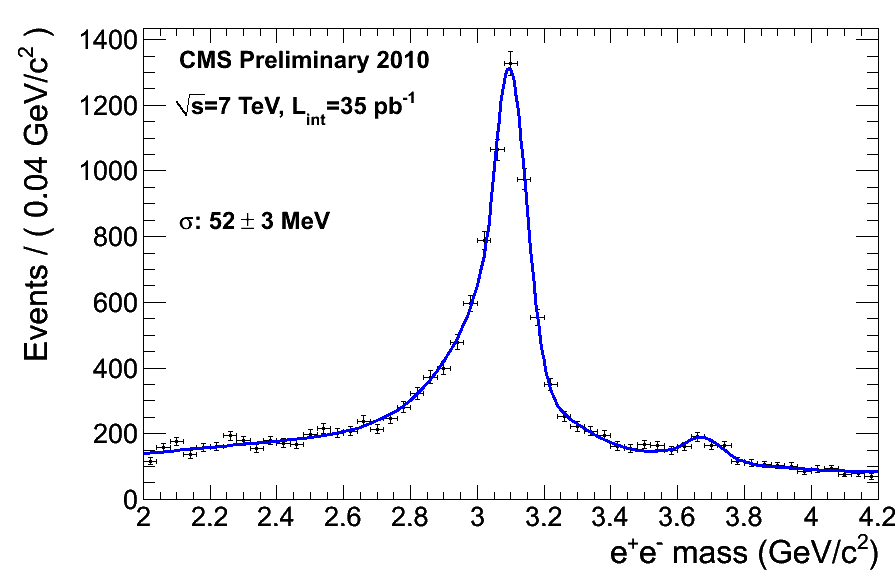
\includegraphics[width=\textwidth]{Figures/Reconstruction_Diagrams/ELE__jpsi_tk_35invpb.png}
        \caption{Reconstructed J$\Psi$ mass peak from di-electron events
          in 7 TeV data, used to commision low \PT electrons reconstructed
        with the particle flow algorithm}\label{fig:ele_jpsi_mass}
      \end{subfigure}
      ~ %add desired spacing between images, e. g. ~, \quad, \qquad, \hfill etc.
      % (or a blank line to force the subfigure onto a new line)
    \begin{subfigure}[h]{0.40\textwidth}
        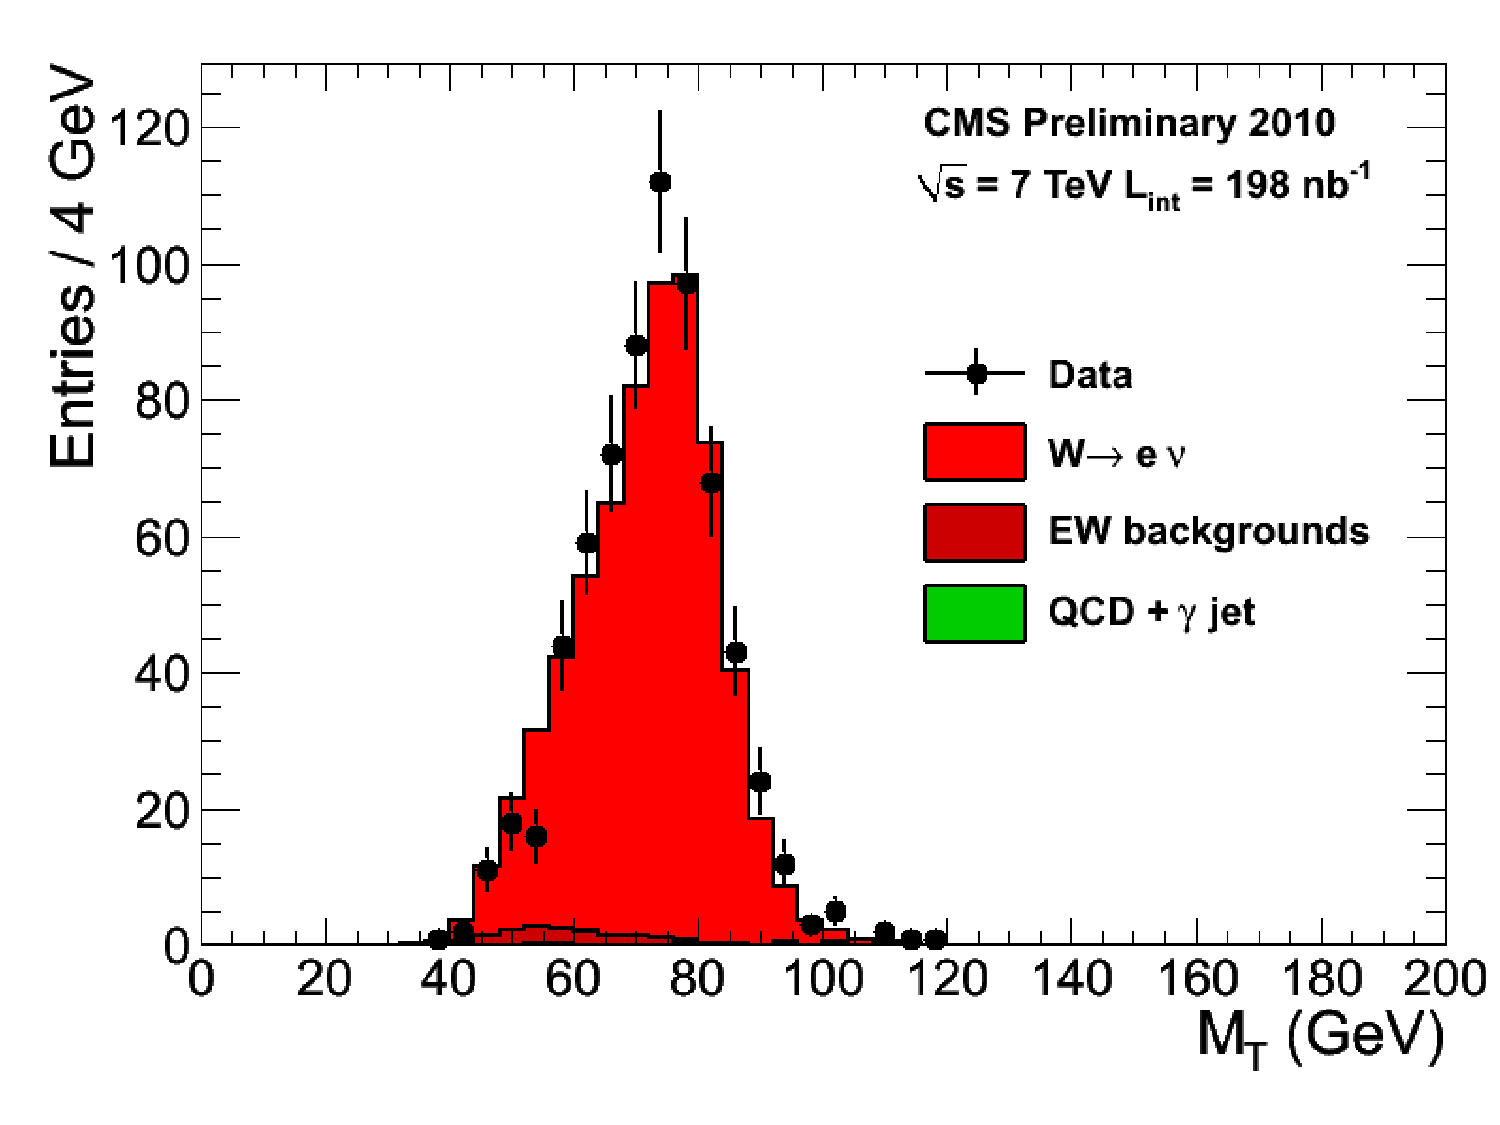
\includegraphics[width=\textwidth]{Figures/Reconstruction_Diagrams/ELE__Welenu_7TeV.pdf}
        \caption{Transverse mass peak of $W$ boson events
          reconstructed from single electron events in 7 TeV data, used to
        commission high \PT electrons reconstructed iwth the particle flow
      algorithm}\label{fig:ele_w_mass}
      \end{subfigure}
      \caption{Electron validation plots for the particle-flow reconstruction}\label{fig:ele_pf_validation}
\end{figure}

\par Similarly to the muons, the electron identification from the
particle-flow algorithm was commisioned using 7 TeV data collected in
2010.  Low \PT electrons were commissioned from the J/$\Psi$ mass
peak, shown in figure
\ref{fig:ele_pf_validation}(\subref{fig:ele_jpsi_mass}) and high \PT
electrons were commissioned from $W$ boson decays, shown in figure
\ref{fig:ele_pf_validation}(\subref{fig:ele_w_mass}). 

\subsection{Charged Hadron Reconstruction}
\label{charged_hadron_reco_overview}

\par Charged hadrons are reconstructed next in the particle flow
algorithm \cite{CMS-PAS-PFT-09-001}.  Tracks linked to both ECAL and
HCAL energy deposits give rise to "particle-flow charged hadrons'' if
calorimeter energy is compatible measured from the curvature of the
tracks in the pixel and silicon detector.  A fit is then performed
between all of the tracks and the HCAL energy clusters to determine an
optimally measured momentum.  In the case where there is only one
track, this fit reduces to a weighted average between the track and
HCAL energy clusters.  

\subsection{Photon and Neutral Hadron Reconstruction}
\label{neutral_hadron_reco_overview}

\par The next step in the algorithm is to identify ECAL and HCAL
energy clusters that aren't linked to tracks or clusters that are
linked to tracks, but have a much larger energy measurement
.  In the latter case, blocks are kept if the
excess energy in the calorimeter clusters is larger than the energy
resolution of the calorimeter.  In both cases, if the total energy
excess in the HCAL is larger than the energy measured in the ECAL,
than a "particle-flow photon'' is created using the energy in the ECAL
and the remaining HCAL energy forms a "particle-flow netural hadron'',
with calibrations performed in the manner described in
sectio \ref{energy_calibration_overview}.  In the case where the ECAL
energy  is larger than the HCAL energy, both cluster energies form a
particle-flow photon.  This is justified the observation that, in jets,
the neutral component of the hadronic energy only deposits 3$\%$ of
the total jet energy in the ECAL, compared to 25$\%$ of the jet energy
from photons.   


\subsection{Jet Reconstruction}
\label{jet_reco_overview}

\par After the formation of photons, charged and neutral hadrons, jets
can be formed by clustering groups of these objects together based on
their momentum weighted, spatial seperation from one another.  This
clustering procedure is performed with the anti-k$_{T}$ algorithm
\cite{Cacciari:2008gp}.   The momentum weighted spatial speration
function between two particles, $i$ and $j$, is defined as:

\begin{equation}\label{eq:antiKt_d}
d_{ij} = \text{min}(\frac{1}{p_{iT}^{2}},
\frac{1}{p_{jT}^{2}})\frac{\Delta_{ij}^{2}}{\text{R}^{2}}
\end{equation}

\noindent where $\Delta_{ij}^{2} =
(y_{i}-y_{j})^{2}+(\phi_{i}-\phi_{j})^{2}$ and $y_{i,j}$ is the
rapidity, and $\phi$ is the azimuthal angle in the CMS detector.  R is
is the distance parameter, which is a user-defined quantitiy for the
algorithm.  

\begin{figure}[h]
   \centering
  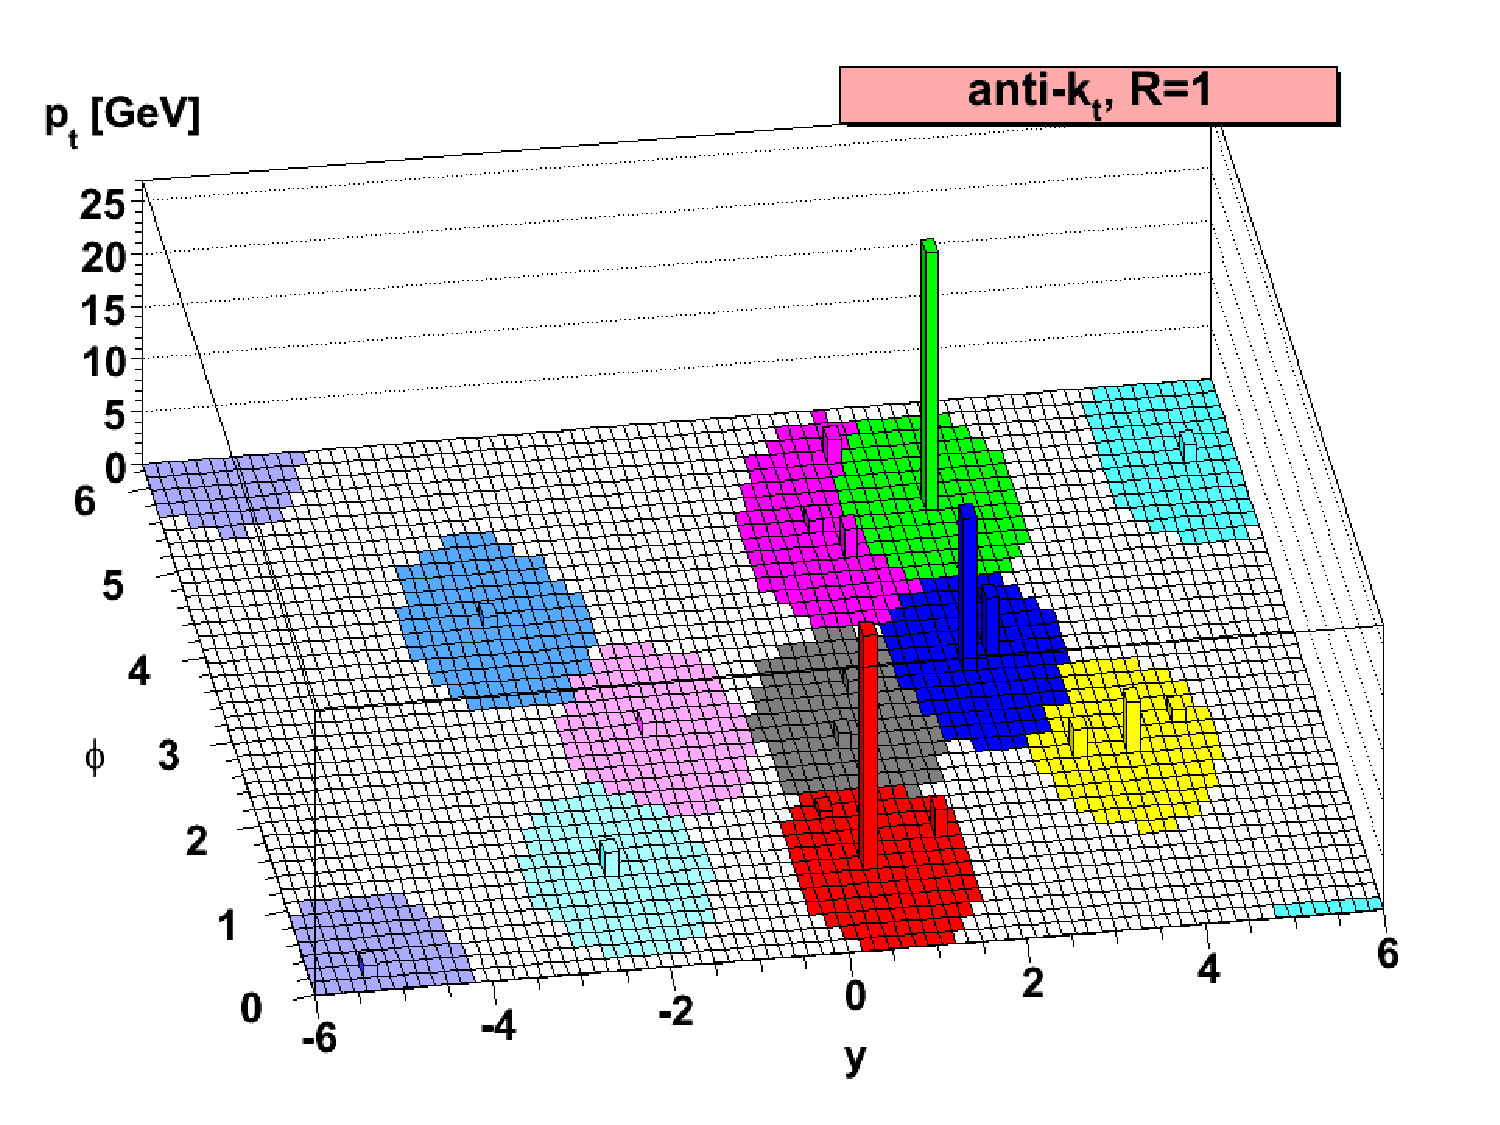
\includegraphics[width=0.8\textwidth]{Figures/Reconstruction_Diagrams/Jets__AntiKt_Algo.pdf}
  \caption{The anti-kt jet clustering algorithm with distance
    parameter R=1.0} \label{fig:antiKt}
\end{figure}

\par The algorithm proceeds by looping over all of the particle-flow
candidate objects that have been formed and calculates the quantity
$d_{ij}$, and combines the two objects with smallest value, into a
single object.  The process is repeated until the smallest value,
$d_{ij}$ has a value $d_{ij} > \frac{1}{p_{Ti}^{2}}$ for all remaining
pairs.  The parameter, $d_{ij}$, will be larger for two small \PT
objects, when compared to a pair of equally spatially separated high
\PT objects.  Thus, softer particles will cluster around harder
objects before clustering amongst themselves.  No hard particles are
present, within the distance parameter, then the object will
accumulate soft particles in a circle of radius R.  The tendency is to
produce circular jets, but in the case where a soft \PT cluster intersects
with a hard \PT cluster, objects the $1/p_{T}^{2}$ weighting will tend
to favor clustering around the harder \PT object.  Figure
\ref{fig:antiKt} shows an example of the results of an anti-kt
algorithm with distance parameter R = 1.0, in the azimuthal-rapitiy
coordinate system.  An example of the preferential grouping around
harder \PT objects can be seen at $\phi=5, y=2$.  

\begin{figure}[h]
   \centering
  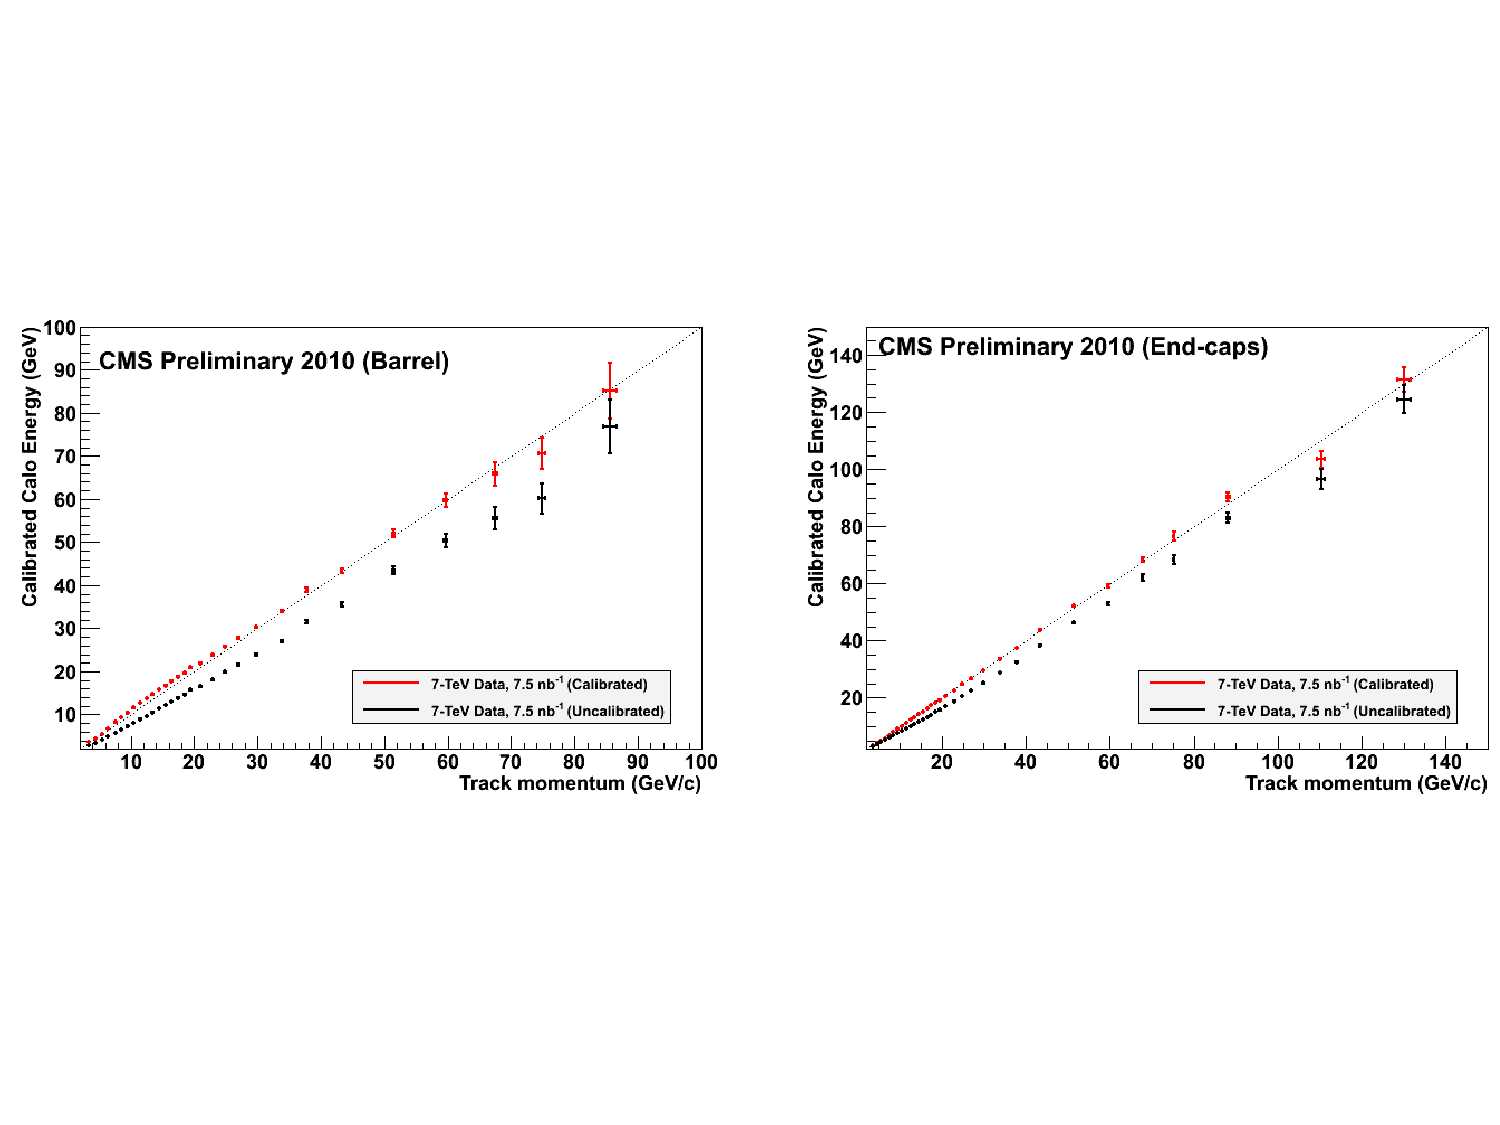
\includegraphics[width=0.8\textwidth]{Figures/Reconstruction_Diagrams/Jets__PFChargedHadronCalibration.pdf}
  \caption{Commissioning of the particle-flow algorithm on jets,
    involved comparing the energy measured from charged hadron tracks,
  to energy measured in calorimeter clusters linked to the tracks} \label{fig:chargedHadron_calib}
\end{figure}

\par In 2010, the particle-flow algorithm for jet reconstruction was
commisioned with 7 TeV data \cite{CMS-PAS-PFT-10-002}.  The
calibration procedure involved selecting charged hadrons from tracks
in the pixel and silicon strip detector, and comparing the energy
measured there to the energy meaured in the calorimeter.  After
calibration, the measurements between tracker and calorimeter agree
within error bars up to 100 GeV, as shown in figure
\ref{fig:chargedHadron_calib}. 

\subsubsection{Hadronic Tau Reconstruction}
\label{tau_reco_overview}

\par Tau leptons are unstable particles which decay via a weak
interaction to lighter particles.  If it decays hadronically via a $W$
boson to two quarks, the tau lepton can be reconstructed analyzing the
resulting jets that are clustered by the anti-kt algorithm.  Tau jets
are characterized by the number of charged hadrons produced in the
decay.  Since charge must be conserved, this results in one charged
hadron being produced $\sim85\%$ of the time, known as a
"one-pronged'' decay, and three charged hadrons being produced
$\sim15\%$ of the time, known as a "three-pronged'' decay.  Thus, a
tau jet is identified as a jet with only 1 or 3 tracks associated with
the calorimeter cluster.  Additionally, the jets from hadronic tau
decays tend to have their energy more collimated than jets produced
from quarks or gluons.  Jets are clusted twice, using two different
distance-parameters.  The ratio of energies of the smaller to the larger of the
distance paramater jets is used to determine how collimated a jet is.
If the ratio is within a given threshold, determined by the analyst in
terms of the reconstruction efficiency and fake rate, the jet is
tagged as a hadronic tau jet. 

\subsubsection{b-Tagging}
\label{b_tagging_overview}

\par Jet that originate from $b$-quarks have unique characteristics
that allow them to be distinguished from jets originating from other
quarks or gluons. This identification process is known as
$b$-tagging.  Several algorithms exist to identify $b$-jets, since
there are many kinematic variables that distinguish them from other
jets.  Due to the heavier nature of the $b$-quark, $b$-jets have
a larger transverse momentum compared to lighter-flavour quarks.
Since it belongs to the third quark generation, it is much more likely
to find a non-prompt lepton embedded in the jet.  Muons are especially
useful to tag $b$-jets since the information they leave in the tracker
can used to easily identify if it came from prompt decay or not.  

\begin{figure}[h]
   \centering
  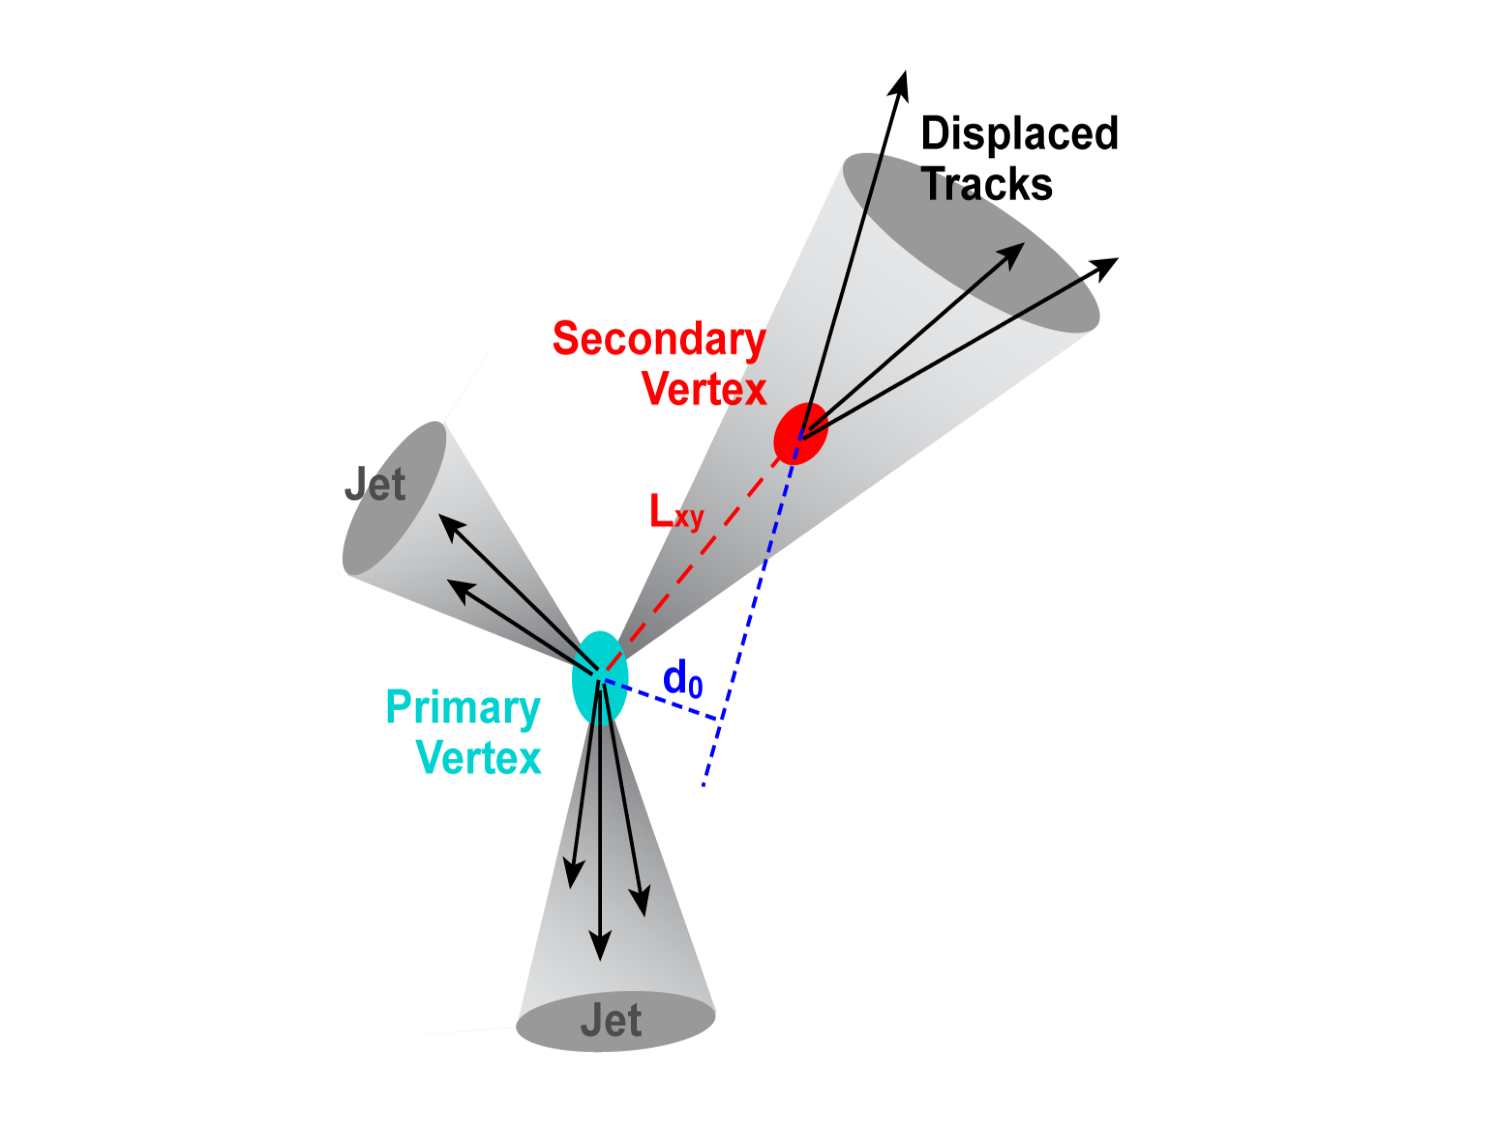
\includegraphics[width=0.6\textwidth]{Figures/Reconstruction_Diagrams/Jets__bTagging.pdf}
  \caption{A $b$-meson will travel a distance L$_{xy}$ before decaying
  and creating a secondary vertex.  The impact parameter, d$_{0}$
  measures the longitudal displacement of the two vertices} \label{fig:bTagging}
\end{figure}

\par The most important characteristic of the $b$-quark is its
relatively long lifetime compared to lighter-flavour quarks.  The
consequence is that a $b$-meson will travel a very small, but
observable distance within the tracker before it decays, forming a
secondary vertex.  The distance and uncertainty measured on the
distance between the primary and secondary vertex is then used as
discriminating variables to tag $b$-jets.  Figure \ref{fig:bTagging}
shows a cartoon of a $b$-jet creating a secondary vertex after
traveling some distance from the primary vertex.   

\subsection{Missing Transverse Energy Reconstruction}

\par CMS has a hermetic design to ensure that all particles produced
in a collision would pass through the detector.  Only long-lived,
neutral particles avoid detection, such as neutrinos in the standard
model.  Many \acrshort{bsm} theories, such as SUSY, are also
characterized by stable, neutral particles.  These particles can only
be detected by measuring a momentum imbalance after measuring all of
the particles in the event.

\par The missing tansverse energy (MET), \ETslash, is the vector sum of
all of particle-flow candidates reconstructed in the event.  It is
defined as 

\begin{equation}\label{eq:met}
\ETslash = | - \sum_{i=1}^{nPF} \vec{p_{Ti}} |
\end{equation}

\noindent where nPF is the number of partice-flow candidates in the
event, and $\vec{p_{Ti}}$ is the vector sum of their transverse
momentum.  

\par The particle-flow alorithm for reconstructing MET was commission
in 2010 with 7 TeV data \cite{CMS-PAS-PFT-10-002}.  Minimum-bias
collisions and QCD multi-jet production are processes that produce no
real MET.  Therefore, a sample of these events were collected,
allowing for the algorithm to be tuned and calibrated.  